\documentclass[11pt]{article}
\usepackage[margin=1in,headheight=24pt]{geometry}
\usepackage{fancyhdr}
\setlength{\headheight}{55pt}
\usepackage{hyperref}
\usepackage{tcolorbox}
\usepackage{xcolor}
\usepackage{amsfonts,amsmath,amssymb,amsthm}
\usepackage{mathtools}
\usepackage{subcaption}
\usepackage{tikz}
\usepackage{tikz-network}

\newtheorem{theorem}{Theorem}[section]
\newtheorem{axiom}[theorem]{Axiom}
\newtheorem{corollary}[theorem]{Corollary}
\newtheorem{definition}[theorem]{Definition}
\newtheorem{example}[theorem]{Example}
\newtheorem{fact}[theorem]{Fact}
\newtheorem{lemma}[theorem]{Lemma}
\newtheorem{proposition}[theorem]{Proposition}
\newtheorem{remark}[theorem]{Remark}

\definecolor{black}{RGB}{0,0,0}
\definecolor{orange}{RGB}{230,159,0}
\definecolor{skyblue}{RGB}{86,180,233}
\definecolor{bluishgreen}{RGB}{0,158,115}
\definecolor{yellow}{RGB}{240,228,66}
\definecolor{blue}{RGB}{0,114,178}
\definecolor{vermillion}{RGB}{213,94,0}
\definecolor{reddishpurple}{RGB}{204,121,167}
\definecolor{cugold}{RGB}{207,184,124}

\pagestyle{plain}

\fancypagestyle{firstpage}{
  \fancyhf{}
  \renewcommand{\headrulewidth}{0pt}
  \fancyhead[c]{
    \makebox[\textwidth][l]{\textbf{MATH 6404: Applied [Combinatorics and] Graph Theory} \hfill CU Denver} \\
    \rule{\textwidth}{0.5pt} \\
    \makebox[\textwidth][l]{Spring 2026 \hfill Instructor: Carlos Mart\'inez}
  }
  \fancyfoot[C]{\thepage}
}

\newcommand{\scribebox}[4]{
\begin{tcolorbox}[colback=cugold!40,colframe=black,left=6pt,right=6pt,top=10pt,bottom=10pt]
    \centering
    \textbf{Lecture #1:} #2 \\
    \textbf{Date:} #3 \hfill     \textbf{Scribe:} #4
\end{tcolorbox}
}


%%% -+-+-+-+-+-+- BEGIN HERE -+-+-+-+-+-+- %%%
\newcommand{\lecturenumber}{$1$}
\newcommand{\lecturetitle}{Introduction}
\newcommand{\scribename}{Carlos Mart\'inez}
\newcommand{\lecturedate}{January 21, 2026}

\begin{document}

\thispagestyle{firstpage}
\scribebox{\lecturenumber}{\lecturetitle}{\lecturedate}{\scribename}

\section{What is Combinatorics?}
To answer this question, we first define a few important sets:
\begin{itemize}
    \item 
    $\mathbb{N} \coloneqq \{1, 2, 3, \ldots\}$ is the set of natural numbers.
    \item
    $\mathbb{Z} \coloneqq \{\ldots, -3, -2, -1, 0, 1, 2, 3, \ldots\}$ is the set of integers.
    \item
    $\mathbb{N}_0 \coloneqq \{0, 1, 2, 3, \ldots\}$ is the set of non-negative integers.
    \item 
    $\mathbb{Q} \coloneqq \{ a/b : a \in \mathbb{Z}, b \in \mathbb{N}
    \}$ is the set of rational numbers.
\end{itemize}

Next, we consider functions.
Let $A$ and $B$ be two sets.
A function $f$ is an assignment of each $a \in A$ to a member of $B$, denoted $f(a) \in B$.
More formally, we write
\begin{equation*}
    \begin{aligned}
    f &:& A &\to B \\
      & & a &\mapsto f(a). 
    \end{aligned}
\end{equation*}
We say that $A$ and $B$ are the domain and co-domain of $f$, respectively.
The set $\{f(a): a \in A\} \subseteq B$ is the image of $f$; in general, this set containment may be strict.

Some functions are nicer than others.
Specifically:
\begin{itemize}
    \item 
    We say $f$ is one-to-one if, for any $a_1, a_2 \in A$, $f(a_1) = f(a_2)$ implies $a_1 = a_2$.
    More formally, $\forall a_1, a_2 \in A$, $f(a_1) = f(a_2) \implies a_1 = a_2$.
    \item 
    We say $f$ is onto if, for any $b \in B$, there exists some $a \in A$ such that $f(a) = b$.
    More formally, $\forall b \in B$, $\exists a \in A$ such that $f(a) = b$.
    \item 
    We say $f$ is a bijection if it is one-to-one and onto.
    If so, we also say that $A$ and $B$ are in bijection.
\end{itemize}
As a general rule, we avoid tedious notation to the extent possible.
In typed writing, it is generally better to write complete sentences.
However, on the whiteboard, we may often recur to tedious notation to save time.
We will see throughout the semester how bijections are nice.

Next, we consider certain properties of sets:
\begin{itemize}
    \item 
    A set $S$ is (infinitely) countable if there is a bijection from $S$ to $\mathbb{N}$.
    For example, the set
    \begin{equation*}
        S = \{\textrm{01/21/26}, \textrm{01/22/26}, \ldots, \textrm{12/31/26}, \textrm{01/01/27}, \ldots \} 
    \end{equation*}
    is countable.
    \item 
    A set $S$ is finite if there is a bijection from $S$ to $[n] \coloneqq \{1, 2, \ldots, n\}$ for some $n \in \mathbb{N}$.
    For example, the set
    \begin{equation*}
        S = \{\textrm{01/01}, \textrm{01/02}, \ldots, \textrm{12/31}\} 
    \end{equation*}
    is finite, as it is in bijection with $[365]$ (assuming a year with $365$ days).
\end{itemize}
Both countable and finite sets are ``discrete.''
Now, to answer the question in a very broad sense:
\begin{center}
    Combinatorics is the study of discrete sets.
\end{center}
Much (if not most) of combinatorics focuses on finite sets, and this will indeed be the focus of this class.
Therefore, unless otherwise stated, all sets we consider are finite.
Combinatorics includes graph theory as a subfield; one that is particularly relevant area because of its broad range of applications.
We will start covering graph theory in short.

\subsection{Two (or Three) Kinds of Questions}
Now, what does the study of finite sets looks like?
In broad strokes, it falls into one of two kinds of questions:
\begin{enumerate}
    \item 
    Given some finite set $S$ specified in some way, how large is it?
    That is, for which $n \in \mathbb{N}$ are $S$ and $[n]$ in bijection?
    This is what it means to ``count.''
    \begin{itemize}
        \item 
        Within this question, a related question is whether the set $S$ as specified is non-empty.
        That is, do objects that meet the specified conditions even exist?
    \end{itemize}
    \item
    Given some (potentially astronomically large) finite set $S$ specified in some way, which of its elements is the ``best'' for some notion of ``goodness''?
    Can one answer this question in a ``reasonable'' amount of time?
    This is what it means to ``optimize.''
\end{enumerate}

Here is an example that foreshadows some of what we will cover in this class (we will introduce formal definitions later).
Consider the graph in Figure~\ref{fig: graph}
\begin{figure}[ht]
    \centering
    \resizebox{0.333\linewidth}{!}{%
        \begin{tikzpicture}
            \Vertex[x=0,y=0,label=$1$]{1}
            \Vertex[x=-2,y=2,label=$2$]{2}
            \Vertex[x=2,y=2,label=$3$]{3}
            \Edge[label=$5$](1)(2)
            \Edge[label=$7$](2)(3)
            \Edge[label=$3$](1)(3)
        \end{tikzpicture}
    }
\caption{A graph.}
\label{fig: graph}
\end{figure}
and its set $S$ of ``spanning trees'' (i.e., connected and acyclic subgraphs) illustrated in Figure~\ref{fig: spanning}.
\begin{figure}[ht]
    \centering
    \begin{subfigure}{0.25\linewidth}
        \resizebox{\linewidth}{!}{%
            \begin{tikzpicture}
                \Vertex[x=0,y=0,label=$1$]{1}
                \Vertex[x=-2,y=2,label=$2$]{2}
                \Vertex[x=2,y=2,label=$3$]{3}
                \Edge[label=$7$](2)(3)
                \Edge[label=$3$](1)(3)
            \end{tikzpicture}
    }
    \end{subfigure}
    \hspace{1cm}
    \begin{subfigure}{0.25\linewidth}
        \resizebox{\linewidth}{!}{%
            \begin{tikzpicture}
                \Vertex[x=0,y=0,label=$1$]{1}
                \Vertex[x=-2,y=2,label=$2$]{2}
                \Vertex[x=2,y=2,label=$3$]{3}
                \Edge[label=$5$](1)(2)
                \Edge[label=$3$](1)(3)
            \end{tikzpicture}
    }
    \end{subfigure}
    \hspace{1cm}
    \begin{subfigure}{0.25\linewidth}
        \resizebox{\linewidth}{!}{%
            \begin{tikzpicture}
                \Vertex[x=0,y=0,label=$1$]{1}
                \Vertex[x=-2,y=2,label=$2$]{2}
                \Vertex[x=2,y=2,label=$3$]{3}
                \Edge[label=$5$](1)(2)
                \Edge[label=$7$](2)(3)
            \end{tikzpicture}
        }
    \end{subfigure}.
\caption{Its spanning trees.}
\label{fig: spanning}
\end{figure}

Then, $|S| = 3$ and the ``best'' element in $S$ is that in Figure~\ref{fig: best}. 
\begin{figure}[ht]
    \centering
    \resizebox{0.25\linewidth}{!}{%
        \begin{tikzpicture}
            \Vertex[x=0,y=0,label=$1$]{1}
            \Vertex[x=-2,y=2,label=$2$]{2}
            \Vertex[x=2,y=2,label=$3$]{3}
            \Edge[label=$5$](1)(2)
            \Edge[label=$3$](1)(3)
        \end{tikzpicture}
    }
\caption{The ``best'' spanning tree.}
\label{fig: best}
\end{figure}
Here, it is the ``best'' in the sense that it has the least total sum of numbers on its edges, with $5 + 3 = 8$.
However, note that there may be other notions of what it means to be the ``best.'' 

Now, for examples as small and simple as this one, it is straightforward enough to answer this question by ``brute force,'' e.g. visual inspection.
Combinatorics is the study of questions like this when the examples are not as simple or small, for which brute force will not work.

\section{What is Graph Theory?}

We now define (unweighted) graphs and some initial graph-theoretic concepts (we will define weighted graphs later).
A graph is a pair $G = (V, E)$ where
\begin{itemize}
    \item 
    $V$ is a set of nodes, where we usually denote $|V| = n$; and
    \item 
    $E$ is a set of edges, where we usually denote $|E| = m$.
    The set of edges is a subset of the cartesian product $V \times V$, i.e. $E \subseteq V \times V = \{(u,v) : u \in V, v \in V\}$.
\end{itemize}
We can now answer the question:
\begin{center}
    Graph theory is the study of graphs.
\end{center}
Let's start studying them!

$E$ is symmetric if $(u, v) \in E$ implies $(v, u) \in E$.
If $E$ is symmetric, we write $\{u, v\} \in E$, with brackets rather than parentheses, to indicate that the order of $u$ and $v$ does not matter.
In this case, we say that $G$ is an undirected graph.
A graph that is not undirected is directed.

Graphs can be drawn in space:
\begin{itemize}
    \item 
    $V$ is drawn as a set of labeled points, e.g. in the plane.
    \item 
    $E$ is drawn as directed or undirected arcs connecting the corresponding points.
\end{itemize}
For example, we can draw the graph $G = (V, E)$ with $V = \{1, 2, 3\}$ and $E = \{\{1,2\}, \{2, 3\}\}$ as in Figure~\ref{fig: undirected}.
\begin{figure}[ht]
    \centering
    \resizebox{0.25\linewidth}{!}{%
        \begin{tikzpicture}
            \Vertex[x=0,y=0,label=$1$]{1}
            \Vertex[x=-2,y=2,label=$2$]{2}
            \Vertex[x=2,y=2,label=$3$]{3}
            \Edge(1)(2)
            \Edge(2)(3)
        \end{tikzpicture}
    }.
\caption{An undirected graph.}
\label{fig: undirected}
\end{figure}

Similarly, we can draw the graph $G = (V, E)$ with $V = \{1, 2, 3\}$ and $E = \{(1,2), (2, 3)\}$ as in Figure~\ref{fig: directed}.
\begin{figure}[ht]
    \centering
    \resizebox{0.25\linewidth}{!}{%
        \begin{tikzpicture}
            \Vertex[x=0,y=0,label=$1$]{1}
            \Vertex[x=-2,y=2,label=$2$]{2}
            \Vertex[x=2,y=2,label=$3$]{3}
            \Edge[Direct](1)(2)
            \Edge[Direct](2)(3)
        \end{tikzpicture}
    }.
\caption{A directed graph.}
\label{fig: directed}
\end{figure}

Note that the drawing of a graph is not the same as the graph itself.
For example, the two drawings in Figure~\ref{fig: drawings} are different but represent the same graph.
\begin{figure}[ht]
    \centering
    \begin{subfigure}{0.25\linewidth}
        \resizebox{\linewidth}{!}{%
            \begin{tikzpicture}
                \Vertex[x=0,y=0,label=$1$]{1}
                \Vertex[x=-2,y=2,label=$2$]{2}
                \Vertex[x=2,y=2,label=$3$]{3}
                \Edge[Direct](1)(2)
                \Edge[Direct](2)(3)
            \end{tikzpicture}
        }
    \end{subfigure}
    \hspace{1cm}
    \begin{subfigure}{0.25\linewidth}
    \centering
    \resizebox{\linewidth}{!}{%
        \begin{tikzpicture}
            \Vertex[x=-2,y=0,label=$1$]{1}
            \Vertex[x=0,y=0,label=$2$]{2}
            \Vertex[x=2,y=0,label=$3$]{3}
            \Edge[Direct](1)(2)
            \Edge[Direct](2)(3)
        \end{tikzpicture}
    }
    \end{subfigure}
\caption{Two different drawings of the same graph.}
\label{fig: drawings}
\end{figure}
However, for ease of presentation, we will often abuse terminology and refer to the drawing of a graph as the graph itself.

\subsection{Graph Isomorphism}
We say two graphs $G = (V(G), E(G))$ and $H = (V(H), E(H))$ are isomorphic if there exists a bijection $\sigma: V(G) \rightarrow V(H)$ such that $(u, v) \in E(G)$ if and only if $(\sigma(u), \sigma(v))) \in E(H)$.
In other words, the bijection must be edge-preserving.

For example, the graphs in Figure~\ref{fig: isomorphic} are isomorphic.
\begin{figure}[ht]
\centering
\begin{subfigure}{0.2\linewidth}
\centering
\resizebox{\linewidth}{!}{%
    \begin{tikzpicture}
        \Vertex[x=0,y=3,label=$a$]{a}
        \Vertex[x=0,y=2,label=$b$]{b}
        \Vertex[x=0,y=1,label=$c$]{c}
        \Vertex[x=0,y=0,label=$d$]{d}
        \Vertex[x=2,y=3,label=$e$]{e}
        \Vertex[x=2,y=2,label=$f$]{f}
        \Vertex[x=2,y=1,label=$g$]{g}
        \Vertex[x=2,y=0,label=$h$]{h}

        \Edge(a)(e)
        \Edge(a)(f)
        \Edge(a)(g)

        \Edge(b)(e)
        \Edge(b)(f)
        \Edge(b)(h)

        \Edge(c)(e)
        \Edge(c)(g)
        \Edge(c)(h)

        \Edge(d)(f)
        \Edge(d)(g)
        \Edge(d)(h)
    \end{tikzpicture}
}
\caption*{$G$}
\end{subfigure}
\hspace{2cm}
\begin{subfigure}{0.2\linewidth}
\centering
\resizebox{\linewidth}{!}{%
    \begin{tikzpicture}
        \Vertex[x=0,y=3,label=$1$]{a}
        \Vertex[x=2,y=2,label=$2$]{b}
        \Vertex[x=1,y=1,label=$3$]{c}
        \Vertex[x=3,y=0,label=$4$]{d}
        \Vertex[x=1,y=2,label=$5$]{e}
        \Vertex[x=3,y=3,label=$6$]{f}
        \Vertex[x=0,y=0,label=$7$]{g}
        \Vertex[x=2,y=1,label=$8$]{h}

        \Edge(a)(e)
        \Edge(a)(f)
        \Edge(a)(g)

        \Edge(b)(e)
        \Edge(b)(f)
        \Edge(b)(h)

        \Edge(c)(e)
        \Edge(c)(g)
        \Edge(c)(h)

        \Edge(d)(f)
        \Edge(d)(g)
        \Edge(d)(h)
    \end{tikzpicture}
}
\caption*{$H$}
\end{subfigure}
\caption{A pair of isomorphic graphs.}
\label{fig: isomorphic}
\end{figure}

To verify this, consider the bijection $\sigma$ with:
\begin{itemize}
    \item 
    $\sigma(a) = 1$, 
    \item $\sigma(b) = 2$, 
    \item $\sigma(c) = 3$, 
    \item $\sigma(d) = 4$, 
    \item $\sigma(e) = 5$, 
    \item $\sigma(f) = 6$, 
    \item $\sigma(g) = 7$, and
    \item $\sigma(h) = 8$.
\end{itemize}


\end{document}
